\subsection{Classifier Performance}
\label{sec:constraintdetection}

Our first experiment evaluates how model and prompt design affect the accuracy of constraint classification. Starting from the prompt in Figure~\ref{fig:classifyprompt} (Section~\ref{sec:classifier}), we derive four
variants by enabling or disabling \emph{constraint examples} and
\emph{table context}: \emph{No Context}, \emph{Table Context},
\emph{Examples}, and \emph{Examples + Table Context}. We evaluate all four variants across six LLMs and all six datasets. Figure~\ref{fig:classifier-results} summarizes the results. Because sentences missed at this stage cannot be recovered later by the mapper, we require a recall of at least 0.90 on every dataset when selecting a default configuration (red dashed line).

\begin{figure}[!ht]
    \centering
    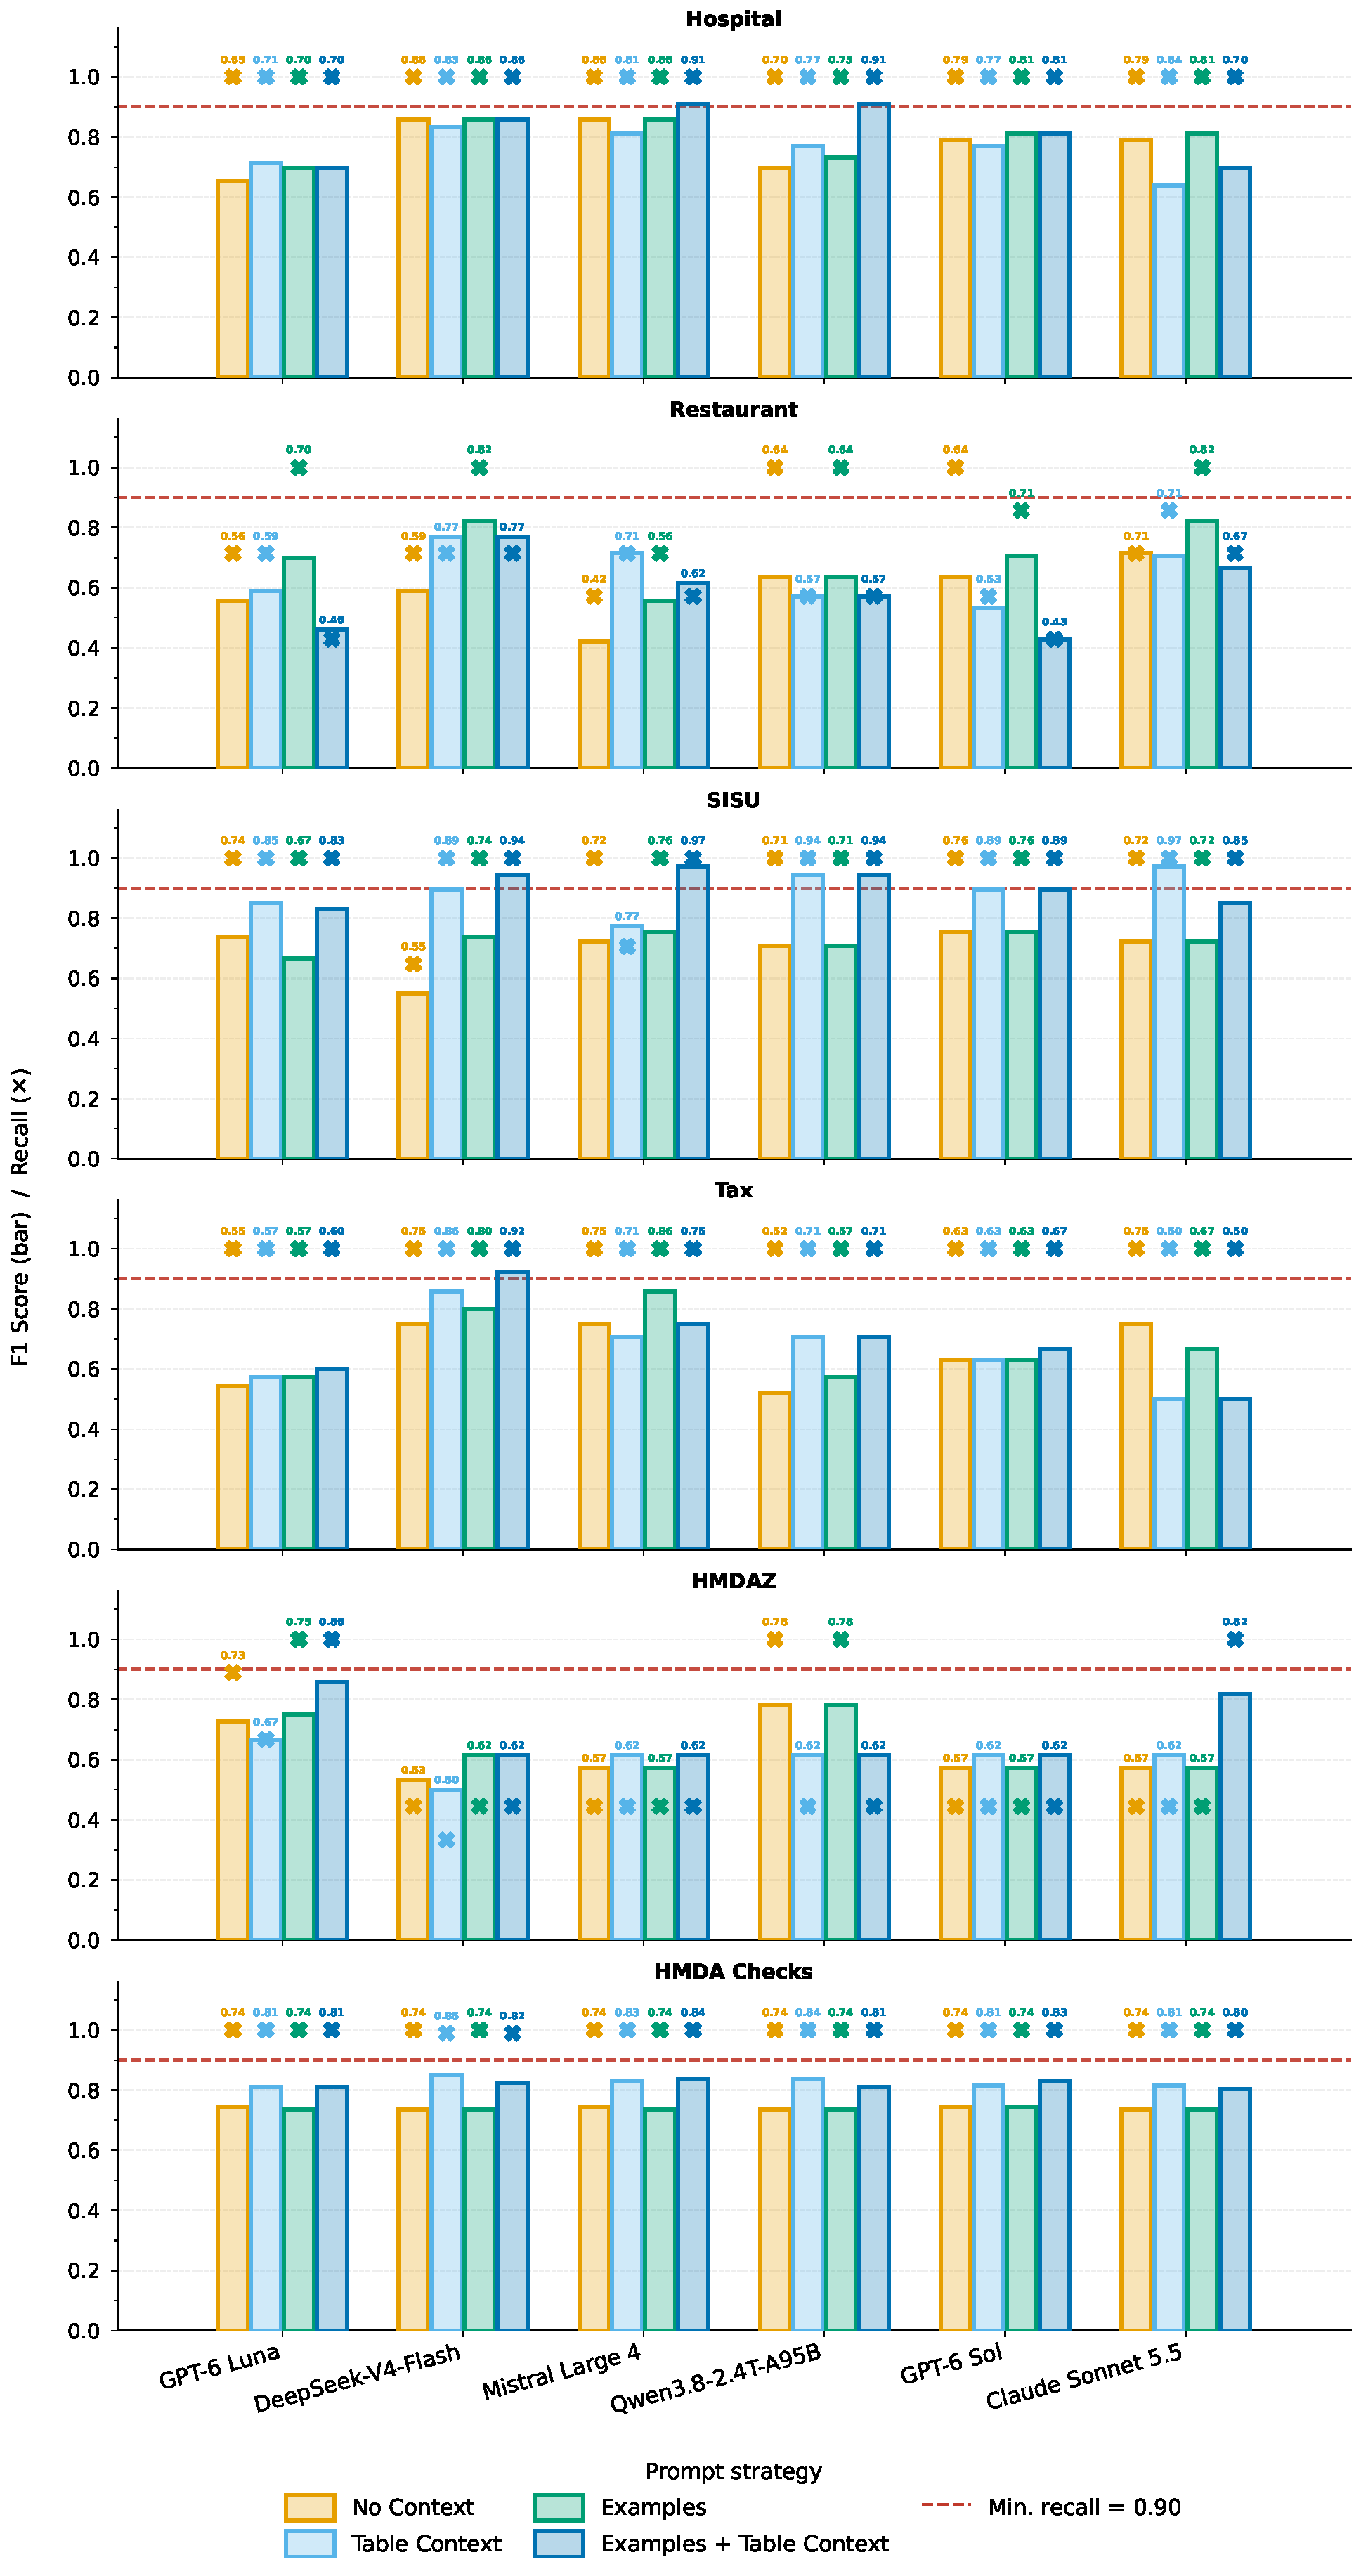
\includegraphics[width=\columnwidth]{figures/results/v3_fig6_classifiers.pdf}
\caption{Constraint classification F$_1$ (bars) and recall (\textsf{x}) across models and prompt variants. The dashed line marks the 0.90 recall threshold.}
    \label{fig:classifier-results}
\end{figure}

On Hospital, Tax, SISU, and HMDA Checks, almost every configuration reaches recall
1.00, so the differences lie in precision. HMDAZ and Restaurant behave
differently: there, recall is the bottleneck. On HMDAZ, most configurations
recover only 4 of the 9 constraint sentences (recall 0.44). The missed sentences
are regulatory definitions (e.g., when a mortgage is high-cost) that read as
scope statements, although each implies a checkable condition on the data. Only three configurations satisfy the recall requirement on all six datasets:
\emph{Qwen3.8-2.4T-A95B} with \emph{Examples} (mean F$_1$ 0.69),
\emph{GPT-6 Luna} with \emph{Examples} (0.69), and \emph{Qwen3.8-2.4T-A95B} with
\emph{No Context} (0.68). As in our previous evaluation, the qualifying configurations
are dominated by \emph{Examples}, and we select \emph{Qwen3.8-2.4T-A95B} with
\emph{Examples} as the default classifier. Configurations with higher mean F$_1$
exist (e.g., DeepSeek-V4-Flash with \emph{Examples + Table Context}, 0.82), but
they miss more than half of the HMDAZ constraints.

Table context has two opposite effects. It is the only signal that raises
precision on HMDA Checks: without it, the models label (almost) every edit as a
constraint, and F$_1$ equals that of the trivial all-positive classifier (0.74).
The non-constraint edits are phrased exactly like the checkable ones and differ
only in that they refer to aggregates, the transmittal sheet, or external
reference data; we conjecture that the record layout shown in the table context
is what lets the model tell them apart. With table context, F$_1$ rises
to 0.80--0.85. On wide schemas, however, the same context does not
help recall: on HMDAZ (135 columns), 9 of the 12 table-context configurations
stay at or below 0.44, and only GPT-6 Luna and Claude Sonnet 5.5 with
\emph{Examples + Table Context} recover all nine constraint sentences. Averaged over all models and datasets, \emph{Examples} gives the best recall (0.93), while the table-context variants give higher precision (0.71 vs.\ 0.58--0.62) at the cost of recall (0.85--0.87).

Compared with the backbones of our previous evaluation, the current models are,
on average, better classifiers on the four original datasets (mean F$_1$ 0.72
vs.\ 0.69 across all configurations), but the best configuration that satisfies
the recall constraint is weaker (0.66 on those four datasets vs.\ 0.85 for
Qwen3-32B with \emph{Examples}). Newer models tend to accept more sentences as
constraints, which keeps recall high but lowers precision, especially on Tax and
Restaurant.
\altic{[R3-O4] Analisar POR QUE o classificador já vai bem sem contexto/exemplos (ganhos marginais, sobretudo no GPT). Discutir a hipótese do revisor: possível exposição a esses datasets/texto regulatório no pré-treino. Mitigar/avaliar: comparar datasets sintéticos vs. SISU/Restaurant, e relacionar com a discussão de vazamento de priors em [R2-O6.2].}
